
\documentclass[journal]{IEEEtran}
%
% If IEEEtran.cls has not been installed into the LaTeX system files,
% manually specify the path to it like:
%\documentclass[journal]{./ieeetrans_template/IEEEtran}


% *** GRAPHICS RELATED PACKAGES ***
%
\ifCLASSINFOpdf
  \usepackage[pdftex]{graphicx}
  % declare the path(s) where your graphic files are
  % \graphicspath{{../pdf/}{../jpeg/}}
  % and their extensions so you won't have to specify these with
  % every instance of \includegraphics
  % \DeclareGraphicsExtensions{.pdf,.jpeg,.png}
\else
  % or other class option (dvipsone, dvipdf, if not using dvips). graphicx
  % will default to the driver specified in the system graphics.cfg if no
  % driver is specified.
  \usepackage[dvips]{graphicx}
  % declare the path(s) where your graphic files are
  % \graphicspath{{../eps/}}
  % and their extensions so you won't have to specify these with
  % every instance of \includegraphics
  % \DeclareGraphicsExtensions{.eps}
\fi
% graphicx was written by David Carlisle and Sebastian Rahtz. It is
% required if you want graphics, photos, etc. graphicx.sty is already
% installed on most LaTeX systems. The latest version and documentation can
% be obtained at: 
% http://www.ctan.org/tex-archive/macros/latex/required/graphics/
% Another good source of documentation is "Using Imported Graphics in
% LaTeX2e" by Keith Reckdahl which can be found as epslatex.ps or
% epslatex.pdf at: http://www.ctan.org/tex-archive/info/
%
% latex, and pdflatex in dvi mode, support graphics in encapsulated
% postscript (.eps) format. pdflatex in pdf mode supports graphics
% in .pdf, .jpeg, .png and .mps (metapost) formats. Users should ensure
% that all non-photo figures use a vector format (.eps, .pdf, .mps) and
% not a bitmapped formats (.jpeg, .png). IEEE frowns on bitmapped formats
% which can result in "jaggedy"/blurry rendering of lines and letters as
% well as large increases in file sizes.
%
% You can find documentation about the pdfTeX application at:
% http://www.tug.org/applications/pdftex


% *** Do not adjust lengths that control margins, column widths, etc. ***
% *** Do not use packages that alter fonts (such as pslatex).         ***
% There should be no need to do such things with IEEEtran.cls V1.6 and later.
% (Unless specifically asked to do so by the journal or conference you plan
% to submit to, of course. )

% correct bad hyphenation here
\hyphenation{op-tical net-works semi-conduc-tor}


\begin{document}

% paper title
% can use linebreaks \\ within to get better formatting as desired
\title{Adaptive MIMO Decoder \\ {\Large EE290C Project Final Report}}

% use \thanks{} to gain access to the first footnote area
% a separate \thanks must be used for each paragraph as LaTeX2e's \thanks
% was not built to handle multiple paragraphs
%

\author{Antonio Puglielli and Simon Scott}


% make the title area
\maketitle

%%%% OBJECTIVES SECTION %%%%
\section{Objectives}

\IEEEPARstart{M}{IMO} refers to the use of multiple transmit antennas {\em and} multiple receive antennas to spatially multiplex data streams over a channel, as illustrated in Figure~\ref{mimo_cartoon}. This channel is often represented by a complex matrix ({\em H}), and can change over time. Although MIMO can be used to increase reliability of a link, this project is only concerned with the use of MIMO to improve throughput. Furthermore, only the single user case will be considered.

The objectives of this project is therefore to develop a MIMO decoder that:
\begin{itemize}
\item supports the antenna configurations and modulation schemes used in both 802.11ac and LTE.
\item meets both the 802.11ac and LTE throughput requirements.
\item is able to adapt to changing channel conditions.
\item is both compile-time and run-time configurable.
\end{itemize}

\begin{figure}[!h]
\centering
\includegraphics*[width=5cm, viewport = 300 0 560 130]{images/agilent_mimo.jpg}
\caption{A 2x2 MIMO configuration}
\label{mimo_cartoon}
\end{figure}


%%%% MOTIVATION AND ALGORITHM SECTION %%%%
\section{Motivation for the LMS Decoding Algorithm}

ANTONIO:
Feel free to write whatever you want here. Essentially, this section will probably be the same as the second slide in our presentation.
Probably also copy some of the text from the motivation section of the project proposal (any references you use should be placed inside the refs.bib file).
Also, feel free to change the title of this section to something more appropriate.


%%%% COMPARISON OF OTHER DECODERS SECTION %%%%
\section{Comparison to other MIMO Decoding Algorithms}
\label{matlab_comparison_section}

ANTONIO:
Compare the MATLAB simulations. Figure \ref{ser_snr_different_schemes_static} is for a static purely random channel. Figure \ref{ser_snr_different_schemes_dynamic} is based on IEEE model B and has 3Hz doppler.

\begin{figure}[!h]
\centering
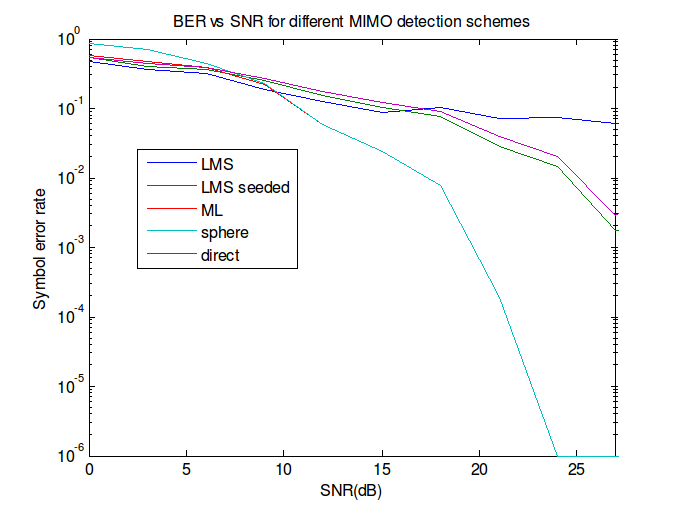
\includegraphics[width=8cm]{images/static_channel_decoder_comparison.png}
\caption{SER vs SNR for different MIMO detection schemes with a static channel}
\label{ser_snr_different_schemes_static}
\end{figure}

\begin{figure}[!h]
\centering
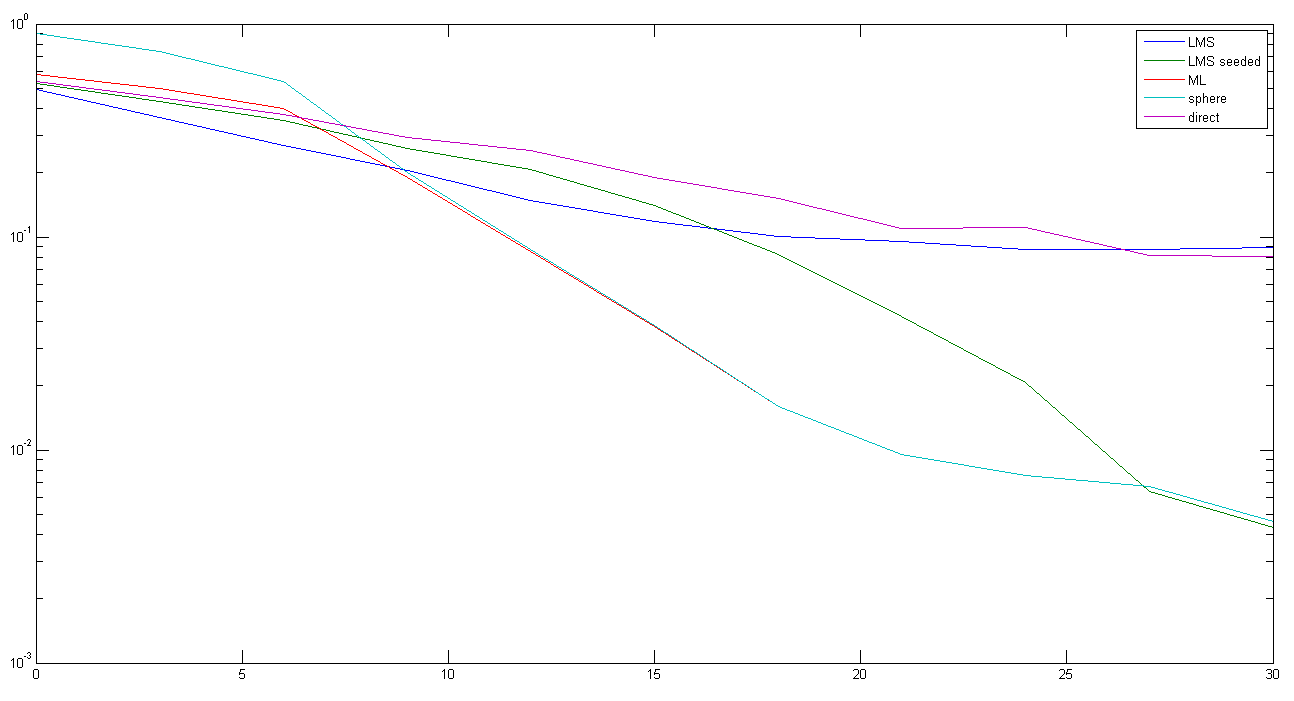
\includegraphics[width=9cm]{images/time_varying_channel_doppler_3.png}
\caption{SER vs SNR for different MIMO detection schemes with a time varying channel (doppler shift of 3Hz)}
\label{ser_snr_different_schemes_dynamic}
\end{figure}


%%%% ARCHITECTURE SECTION %%%%
\section{Hardware Architecture}

SIMON: overview description of hardware.

\begin{figure}[!h]
\centering
\includegraphics*[width=9cm, viewport = 0 90 789 600]{images/top_level_arch.pdf}
\caption{The hardware architecture of the LMS Adaptive MIMO Decoder}
\label{top_level_arch}
\end{figure}

\subsection{Matrix Engine}

SIMON

\begin{figure}[!h]
\centering
\includegraphics*[width=4cm, viewport = 30 640 260 840]{images/matrix_engine.pdf}
\caption{Design of the matrix engine}
\label{matrix_engine}
\end{figure}

\subsection{Channel Estimator Module}

ANTONIO

\subsection{Initialize Weights Module}

ANTONIO

\subsection{Adaptive Decoder Module}

SIMON

\begin{figure}[!h]
\centering
\includegraphics*[width=8cm, viewport = 0 510 560 810]{images/adaptive_decoder.pdf}
\caption{The adaptive decoder module}
\label{adaptive_decoder}
\end{figure}

\subsection{Evaluation of Bitwidths}

The LMS MIMO Decoder architecture described above was implemented in Chisel \cite{chisel}. In order to verify correctness and determine the optimum bitwidths to use, the design was tested in Chisel, using test vectors taken from the MATLAB simulations (as described in Section \ref{matlab_comparison_section}). The symbol error rate versus SNR plots for different bitwidths, for a static channel, are shown in Figure~\ref{ser_ber_chisel_static}. This plot also includes the results from the MATLAB simulation for comparison. Similarly, Figure~\ref{ser_ber_chisel_dynamic} shows the SER vs SNR plots for a slowly changing channel.

\begin{figure}[!h]
\centering
\includegraphics*[width=8cm, viewport = 80 260 560 530]{images/snr_ber_curves_chisel_static.pdf}
\caption{SER vs SNR curves for Chisel implementations with different bitwidths (static channel)}
\label{ser_ber_chisel_static}
\end{figure}

\begin{figure}[!h]
\centering
\includegraphics*[width=9cm, viewport = 80 270 560 530]{images/snr_ber_curves_chisel_doppler.pdf}
\caption{SER vs SNR curves for Chisel implementations with different bitwidths (dynamic channel)}
\label{ser_ber_chisel_dynamic}
\end{figure}

For the static channel, the 20 bit and 24 bit Chisel implementations very closely track the MATLAB simulations, while the 16 bit simulation is completely incorrect. However, for the dynamic channel, where higher precision is needed to track the changing channel, only the 24 bit implementation is able to match the performance of the MATLAB simulation. Therefore, 24 bits was selected as the desired bitwidth for the design.

The poor performance at lower bitwidths is caused by arithmetic overflow during the matrix inverse operation in the Initialize Weights module. Since the channel matrix H can be poorly conditioned, the entries in its inverse matrix can have a high dynamic range, resulting in arithmetic overflow if too few bits are used. Better performance can be achieved at lower bitwidths if saturating arithmetic or pseudo-floating-point were used. Unfortunately, neither of these two features are currently supported in Chisel.


%%%% SYNTHESIS CONSTRAINTS SECTION %%%%
\section{Synthesis Options and Constraints}

SIMON:
Throughput requirement
Levels of parallelism
Latency of seeding matrix, based on 802.11ac specs.


%%%% SYNTHESIS RESULTS SECTION %%%%
\section{Synthesis Results}

SIMON:
Clock, area power
Power breakdown
Can achieve better results if voltage scale.

ANTONIO: if you can, please insert some 2x2 vs 4x4 results here. Mention that 4x4 hardware supports 2x2, but more efficient to generate 2x2 hardware.

ANTONIO: do we want to compare to area/power of other MIMO decoders from the literature?

\begin{figure}[!h]
\centering
\includegraphics*[width=8cm, viewport = 60 250 560 540]{images/power_vs_area.pdf}
\caption{Power vs area for different levels of parallelism}
\label{power_vs_area}
\end{figure}

SIMON:
Conclusion: better performance if faster clock and take many cycles in MAtrix Engine.

\begin{figure}[!h]
\centering
\includegraphics*[width=6cm, viewport = 90 100 660 540]{images/power_breakdown_module.pdf}
\caption{Power of LMS MIMO Decoder by module}
\label{power_breakdown_module}
\end{figure}

SIMON:
Power gating will clearly help, as shown in table below.

\begin{table}[!h]
\caption{Breakdown of power by module}
\label{power_breakdown_table}
\centering
\begin{tabular}{l l l r}
\hline
Module & Submodule & & Power (mW) \\
\hline
Adaptive Decoder & & & 15.1 \\
Initialize Weights & Mat4 Inverse & 3.96 & \\
 & Mat2 Inverse & 24.8 & \\
 & Module total & & 33.7 \\
Channel Estimator & & & 2.13 \\
Matrix Engine & & & 25.4 \\
Queues & & & 1.81 \\
\hline
\em{Total} & & & \em{78.14} \\
Total without & & & \\
initialization modules & & & 42.31 \\
\hline
\end{tabular}
\end{table}


%%%% CONCLUSION AND FUTURE WORK SECTION %%%%
\section{Conclusions and Future Work}

ANTONIO: I'll leave this for you to fill out once you've finished your section.

Things to mention: power gating of initialization modules; adjusting mu (LMS step size) dynamically; producing soft decisions and then adjusting weights based on hard decisions from LDPC decoder; voltage scaling as we reduce the clock rate for higher levels of parallelization; pseudo-floating point or saturating arithmetic in inverse engine to allow fewer bits to be used.


% references section

\bibliographystyle{IEEEtran}
\bibliography{refs}

\end{document}


